% coding:utf-8

%FOSASTOC, a LaTeX-Code for a electrical summary of stochastic
%Copyright (C) 2013, Daniel Winz, Ervin Mazlagic

%This program is free software; you can redistribute it and/or
%modify it under the terms of the GNU General Public License
%as published by the Free Software Foundation; either version 2
%of the License, or (at your option) any later version.

%This program is distributed in the hope that it will be useful,
%but WITHOUT ANY WARRANTY; without even the implied warranty of
%MERCHANTABILITY or FITNESS FOR A PARTICULAR PURPOSE.  See the
%GNU General Public License for more details.
%----------------------------------------

\chapter{Diskrete Verteilungen}
Diskrete Verteilungen beschreiben Probleme, welche
Ergebnisse aus $\mathbb{N}$ liefern und binär sind.

\paragraph{Binär}
Binär bedeutet, dass ein Ereignis zwei Werte annehmen kann. Bekannte
Beispiele binärer Probleme sind
\begin{itemize}
	\item Gewinnlose \hfill{} (\emph{Gewinn, Zonk})
	\item Münzwurf \hfill{} (\emph{Kopf, Zahl})
	\item Telefon \hfill{} (\emph{klingelt, klingelt nicht})
\end{itemize}
Viele nicht-binäre Probleme können aber leicht in binäre gewandelt
werden. Beispielsweise liefert ein Sensor analoge Signale, diese sind
$\notin \mathbb{N}$ noch sind diese binär. 
Dennoch kann man das Signal binär
untersuchen mit der Fragestellung 
"`\emph{Ist der Wert grösser als $xy$?}"'.
Diese Frage kann semantisch nur mit \emph{Ja} und \emph{Nein} beantwortet
werden und beschreibt somit ein binäres Problem. Die Zahl der Antworten
kann wiederum nur $\in \mathbb{N}$ sein. Somit sind die Bedingungen 
für ein binäres Problem gegeben.

\newpage
\section{Hypergeometrische Verteilung}
Die hypergeometrische Verteilung entspricht dem Urnenmodell:
\begin{itemize}
	\item Urne hat $r$ rote (postive) und $s$ schwarze (negative)
		Kugeln
		\[ r,s \in \mathbb{N} \]
	\item Die Menge der roten als auch der schwarzen Kugeln ist fix 
		\[ r,s \neq \infty \]
	\item Ein erzieltes Ergebnis reduziert die entsprechende Menge
		(\emph{Ziehen ohne Zurücklegen})
		\[ r \rightarrow  R - 1\]
\end{itemize}

\subsection{Verteilungsfunktion}
\[  
	X \sim Hyp(n,r,s)
\]

\[ \begin{array}{c l}
	n & \text{Anzahl Ziehungen} \\
	r & \text{Anzhal roter Kugeln (positive Ereignisse)} \\
	s & \text{Anzahl blauer Kugeln (negative Ereignisse)} \\
	N & \text{Anzahl Kugeln in der Urne } (N=r+s)
\end{array} \]

\[
	P(X=k)
		= \frac{\displaystyle 
			\binom{r}{k} \cdot \binom{s}{n-k}}{
				\displaystyle \binom{r+s}{n}}
		= \frac{\displaystyle 
			\binom{r}{k} \cdot \binom{N-r}{n-k}}{
				\displaystyle \binom{N}{n}}
\]

\subsection{Erwartungswert}

\[ 
	E(X) = n \cdot \frac{r}{N}, \qquad X \sim Hyp(n,r,s)
\]

\subsection{Varianz}

\[  
	Var(X) = n \cdot \frac{r}{N} \cdot 
		\left(1 - \frac{r}{N} \right)
		\cdot \frac{N-n}{N-1}, \qquad X \sim Hyp(n,r,s)
\]

\subsection{Verwendung in R}
\lstinline{R} stellt grundsätzlich vier Funktionen für die 
hypergeometrische Verteilung zur Verfügung. 
\begin{itemize}
	\item \lstinline{dhyper()} \hfill{} 
		(\emph{Wahrscheinlichkeitsverteilung})
	\item \lstinline{phyper()} \hfill{}
		(\emph{kumulative Wahrscheinlichkeit})
	\item \lstinline{qhyper()} \hfill{}
		(\emph{Verteilung der Quantile})
	\item \lstinline{rhyper()} \hfill{}
		(\emph{Zufallszahlen})
\end{itemize}
Die Abbildung \ref{fig:hyper} zeigt jeweils einen Plot zu den gegebenen
Funktionen aus \lstinline{R}. Für weitere Informationen zu Plots siehe
Kapitel \ref{sec:plots}.





\begin{figure}[h!]
\centering
\begin{subfigure}[b]{0.48\textwidth}
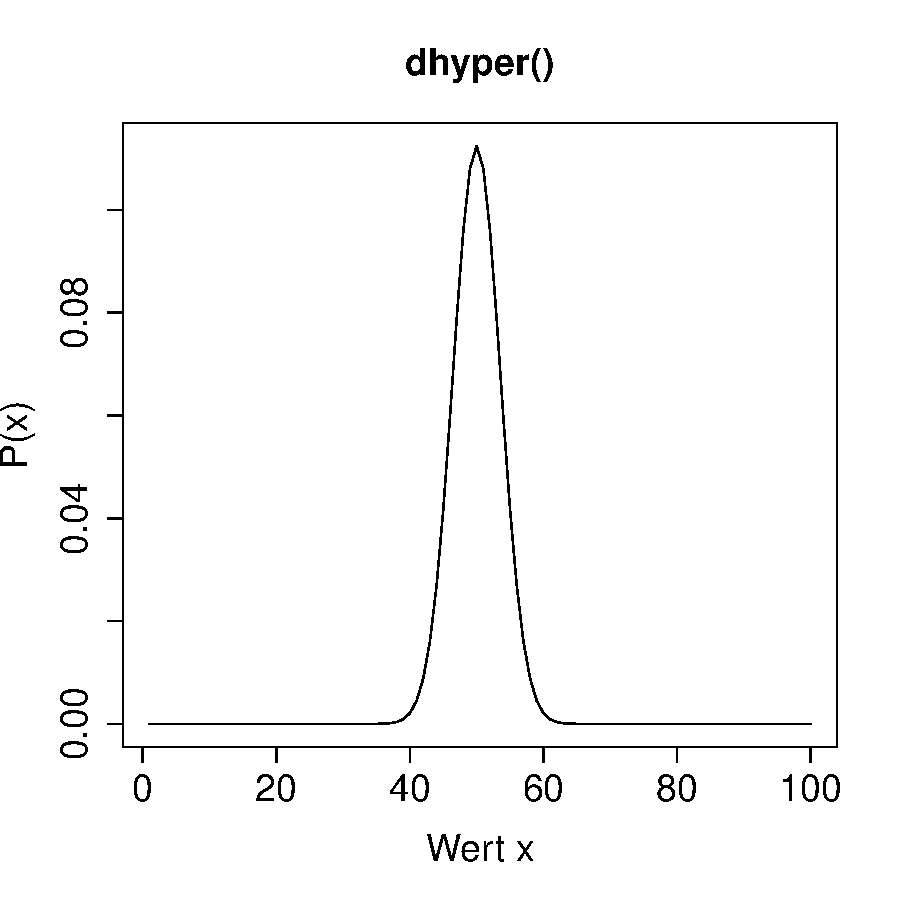
\includegraphics{verteilungen-005}
\caption{Wahrscheinlichkeitsverteilung}
\end{subfigure}
\begin{subfigure}[b]{0.48\textwidth}
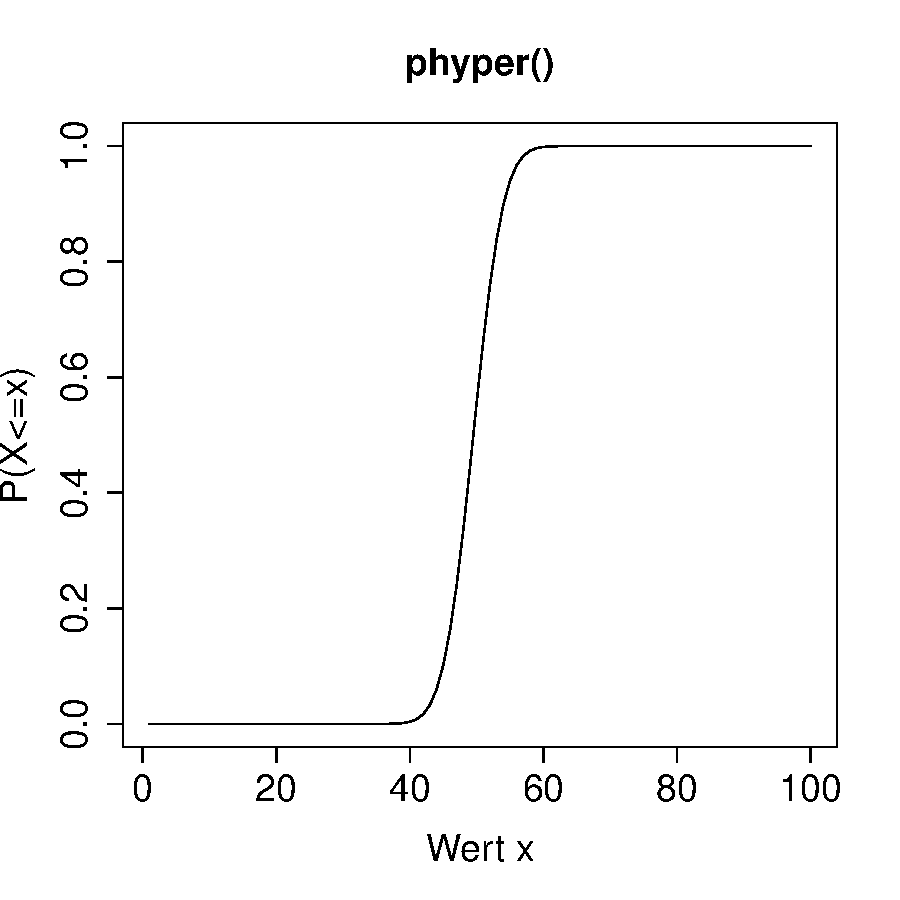
\includegraphics{verteilungen-006}
\caption{kumulative Wahrscheinlichkeit}
\end{subfigure}

\begin{subfigure}[b]{0.48\textwidth}
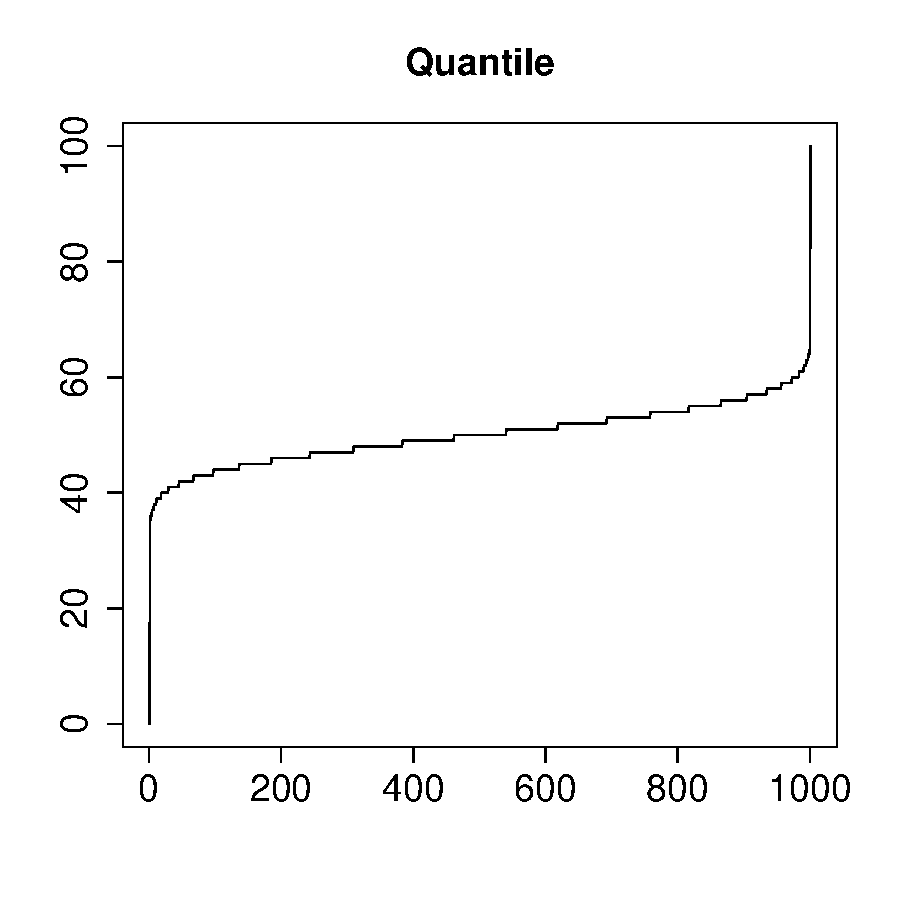
\includegraphics{verteilungen-007}
\caption{Quantile}
\end{subfigure}
\begin{subfigure}[b]{0.48\textwidth}
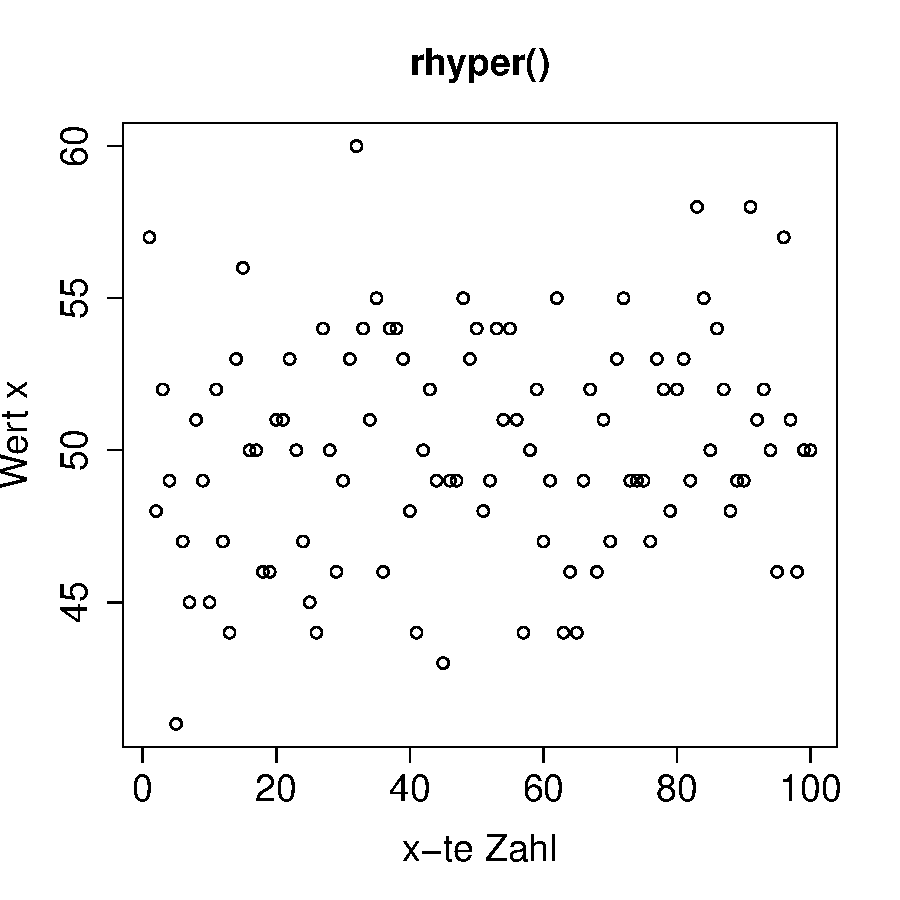
\includegraphics{verteilungen-008}
\caption{Zufallszahlen}
\end{subfigure}
\caption{Hypergeometrische Verteilung ($m=100, n=100, k=100$)}
\label{fig:hyper}
\end{figure}

\clearpage

\subsection{Beispiel einer hypogeometrischen Verteilung}
Ein Beispiel aus dem Alltag ist die Teambildung im Mannschaftssport.
Ein Turnverein hat $9$ männliche und $17$ weibliche Mitglieder. Für ein
Fussballmatch gegen einen anderen Verein muss nun ein Team mit $11$
Mitgliedern gebildet werden. Wie wahrscheinlich ist es, dass das
Team aus einer bestimmten Anzahl Männern oder Frauen besteht?
\paragraph{Berechnung in R}
\begin{Schunk}
\begin{Sinput}
> man <- 9; women <- 17; player <- 11
> boys <- dhyper(x=c(1:player), m=man, n=women, k=player)
> girls <- dhyper(x=(1:player), m=women, n=man, k=player)
> plot(boys, type='h')
> plot(girls, type='h')
\end{Sinput}
\end{Schunk}
\begin{figure}[h!]
\centering
\begin{subfigure}[b]{0.48\textwidth}
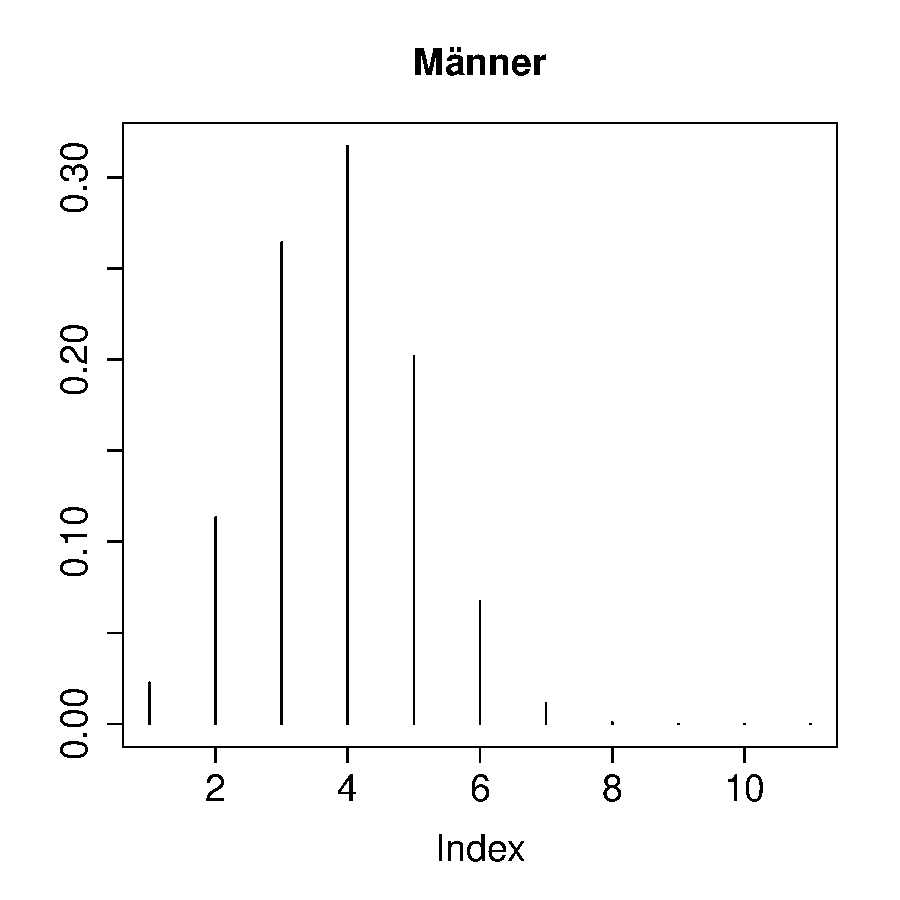
\includegraphics{verteilungen-012}
\caption{$P(x)$ der Männer im Team}
\end{subfigure}
\begin{subfigure}[b]{0.48\textwidth}
\centering
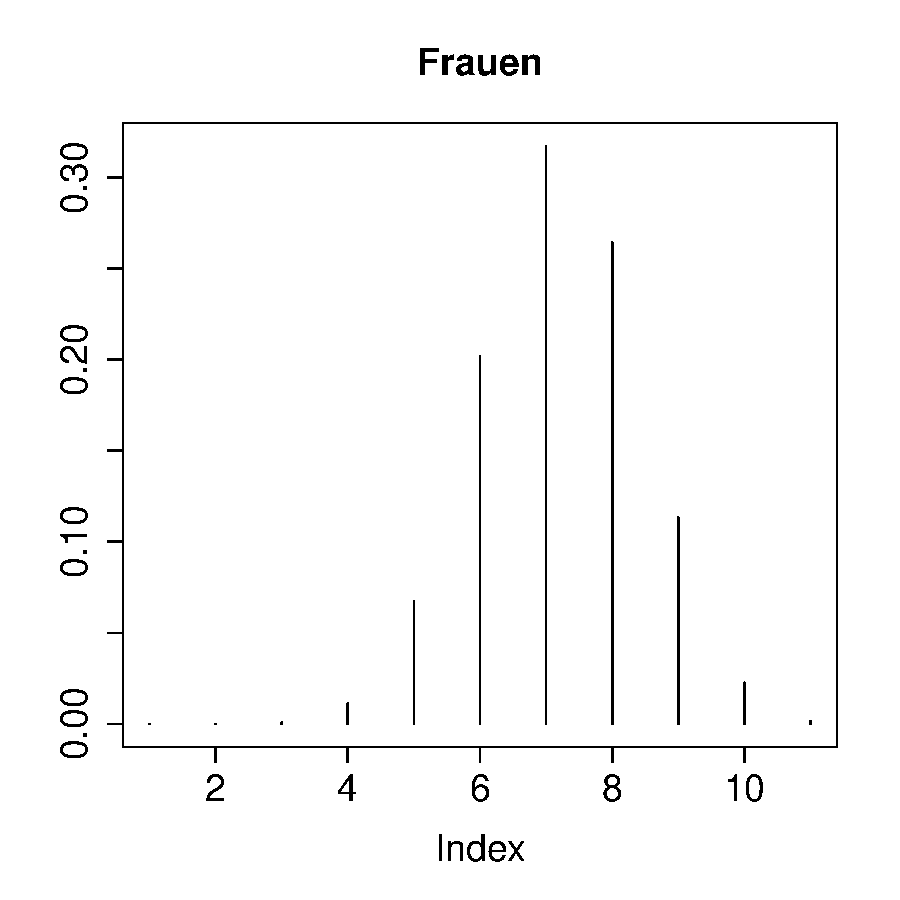
\includegraphics{verteilungen-013}
\caption{$P(x)$ der Frauen im Team}
\end{subfigure}
\caption{Teambildung nach Geschlecht}
\label{fig:team}
\end{figure}

\noindent
Die Plots aus der Abbildung \ref{fig:team} zeigen, dass es mit der 
höchsten Wahrscheinlichkeit
4 Männer und 7 Frauen im Team hat, was die gewünschte Anzahl von Spielern
ergibt für das Team ($4+7=11$). 

\clearpage
\newpage
\section{Binomialverteilung}
Die Binomialverteilung ist eine Verteilung, welche bei binären Problemen
auftritt wobei ein erzieltes Ergebnis nicht die weiteren Ergebnisse
beeinflusst. Sie ist somit ein Grenzfall der hypergeometrischen 
Verteilung (nämlich dann, wenn es sehr viele rote und schwarze 
Kugeln gibt).
\[ 
	\lim_{r,s \rightarrow \infty} Hyp(n,r,s) 
	\quad \Rightarrow \quad Bin(n,p)
\]

\subsection{Verteilungsfunktion}

\[ 
	X \sim Bin(n,p)
\]

\[ \begin{array}{c l} 
	n & \text{Anzahl Versuche} \\
	p & \text{Trefferwahrscheinlichkeit}
\end{array} \]

\[ \begin{array}{l c l} 
	P(X=x)
		&= 
		& \displaystyle \binom{n}{x} \cdot p^x 
			\cdot (1-p)^{n-x} \\
	& & \\
		&= 
		& \frac{\displaystyle n!}{\displaystyle x!\, (n-x)!} 
			\cdot p^x \cdot (1-p)^{n-x}
\end{array} \]

\subsection{Erwartungswert}

\[  
	E(X) = n \cdot p, \qquad X \sim Bin(n,p)
\]


\subsection{Varianz}

\[  
	Var(X) = n \cdot p \cdot (1-p), \qquad X \sim Bin(n,p)
\]

\subsection{Verwendung in R}
\lstinline{R} stellt grundsätzlich vier Funktionen für die 
Binomialverteilung zur Verfügung. 
\begin{itemize}
	\item \lstinline{dbinom()} \hfill{} 
		(\emph{Wahrscheinlichkeitsverteilung})
	\item \lstinline{pbinom()} \hfill{}
		(\emph{kumulative Wahrscheinlichkeit})
	\item \lstinline{qbinom()} \hfill{}
		(\emph{Verteilung der Quantile})
	\item \lstinline{rbinom()} \hfill{}
		(\emph{Zufallszahlen})
\end{itemize}
Die Abbildung \ref{fig:binom} zeigt jeweils einen Plot zu den gegebenen
Funktionen aus \lstinline{R}. Für weitere Informationen zu Plots siehe
Kapitel \ref{sec:plots}.





\begin{figure}[h!]
\centering
\begin{subfigure}[b]{0.48\textwidth}
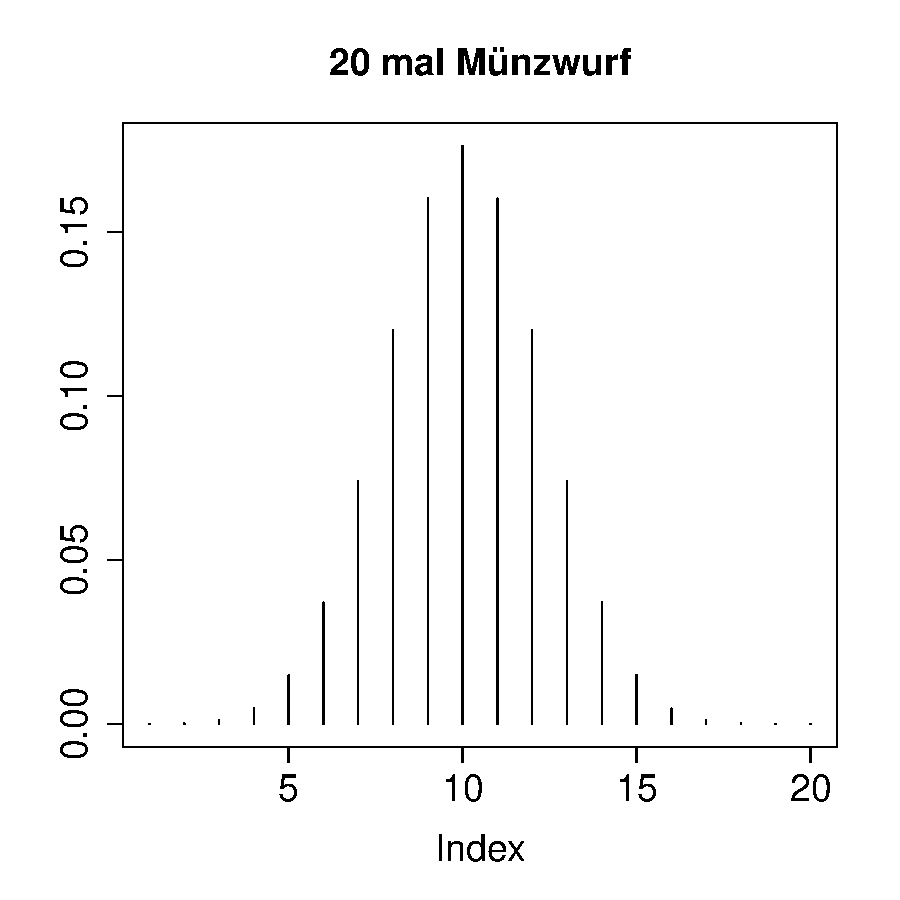
\includegraphics{verteilungen-018}
\caption{Wahrscheinlichkeitsverteilung}
\end{subfigure}
\begin{subfigure}[b]{0.48\textwidth}
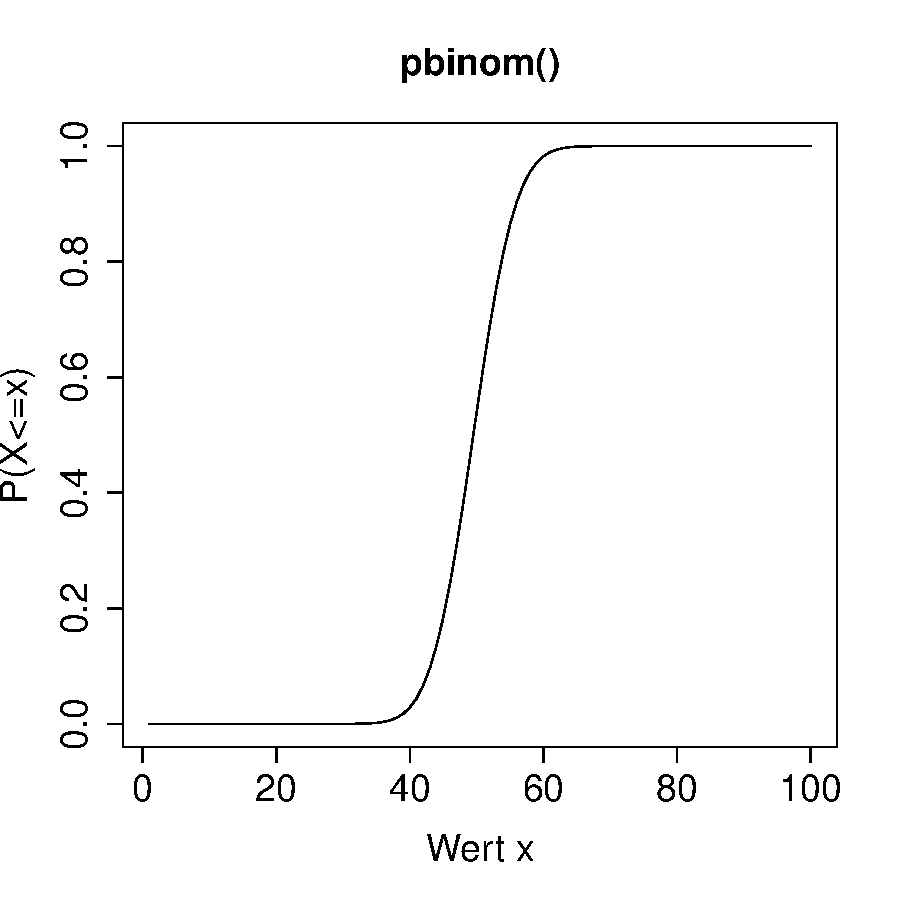
\includegraphics{verteilungen-019}
\caption{kumulative Wahrscheinlichkeit}
\end{subfigure}

\begin{subfigure}[b]{0.48\textwidth}
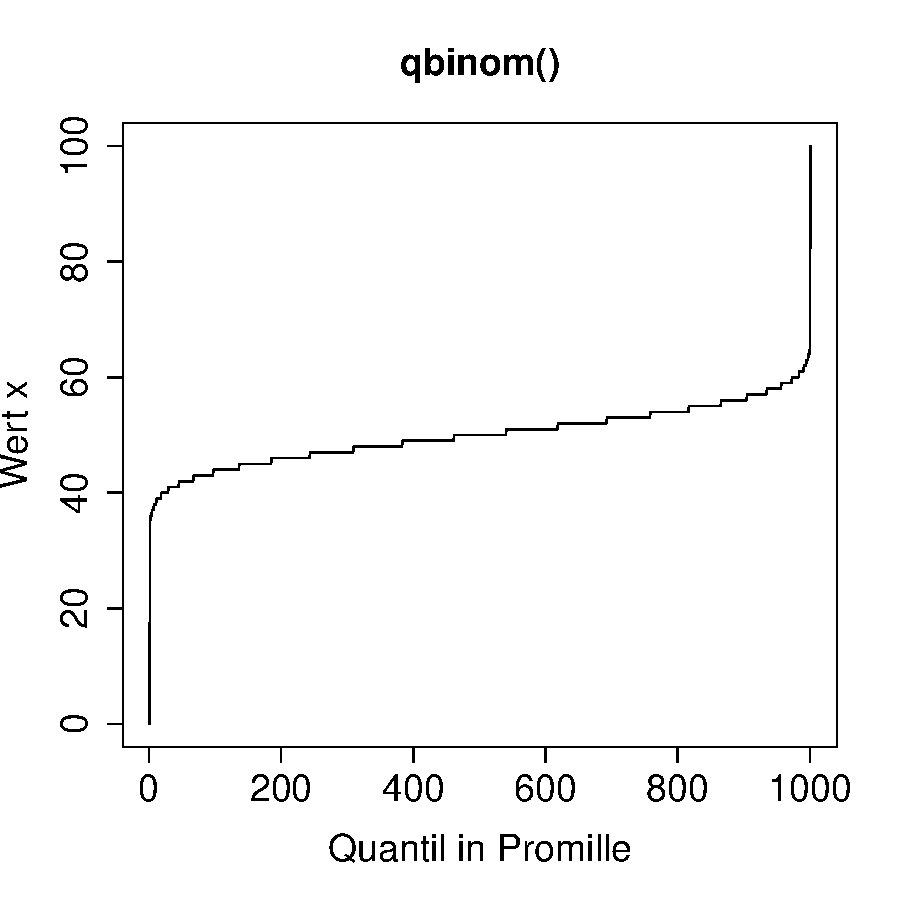
\includegraphics{verteilungen-020}
\caption{Quantile}
\end{subfigure}
\begin{subfigure}[b]{0.48\textwidth}
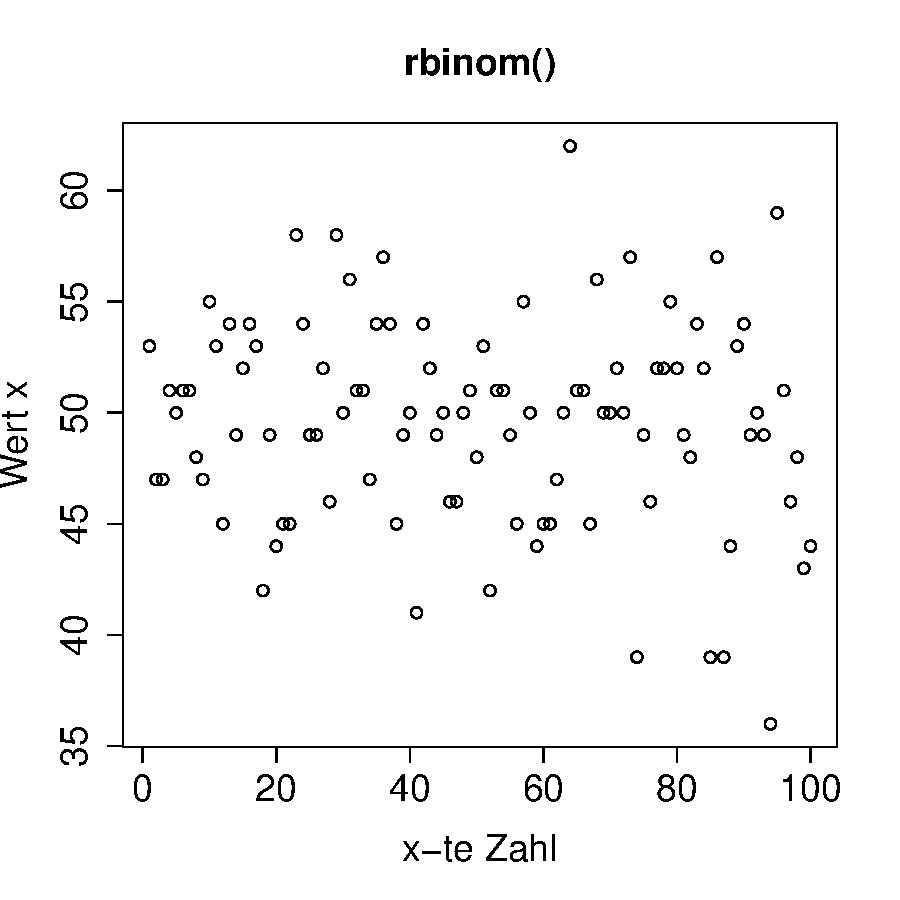
\includegraphics{verteilungen-021}
\caption{Zufallszahlen}
\end{subfigure}
\caption{Binomialverteilung ($n=100, p=0.5$)}
\label{fig:binom}
\end{figure}

\subsection{Beispiel einer binomialen Verteilung}
Jemand sagt Ihnen, dass er von 100 Münzwürfen 80 mal Kopf erhielt.
Sie antworten spontan, dass Sie ihm 15 Treffer von 20 Versuchen ja 
noch geglaubt hätten aber nicht 80 von 100. 
Wie wahrscheinlich sind aber diese beiden Ergebnisse wenn Kopf 
und Zahl jeweils gleichwahrscheinliche Ergebnisse sind?

\begin{Schunk}
\begin{Sinput}
> plot(dbinom(x=c(1:100), size=100, prob=0.5), type='h')
> plot(dbinom(x=c(1:20), size=20, prob=0.5), type='h')
\end{Sinput}
\end{Schunk}


\begin{figure}[h!]
\centering
\begin{subfigure}[b]{0.48\textwidth}
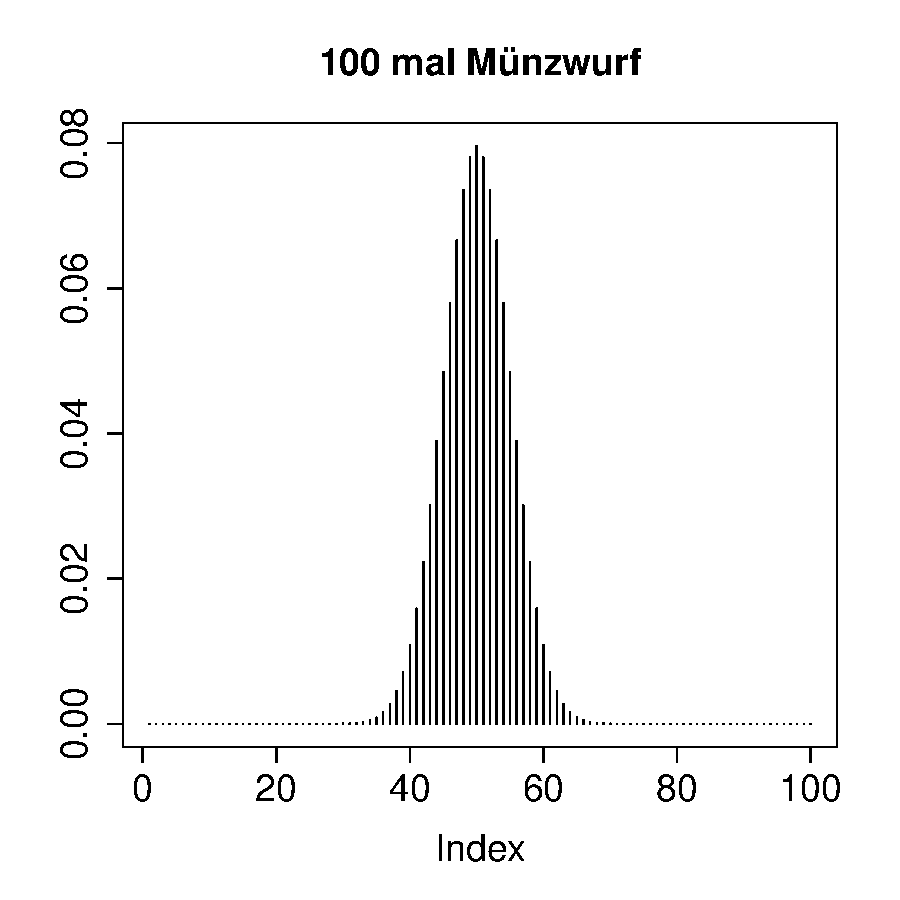
\includegraphics{verteilungen-025}
\caption{Verteilung für 100 Versuche}
\end{subfigure}
\begin{subfigure}[b]{0.48\textwidth}
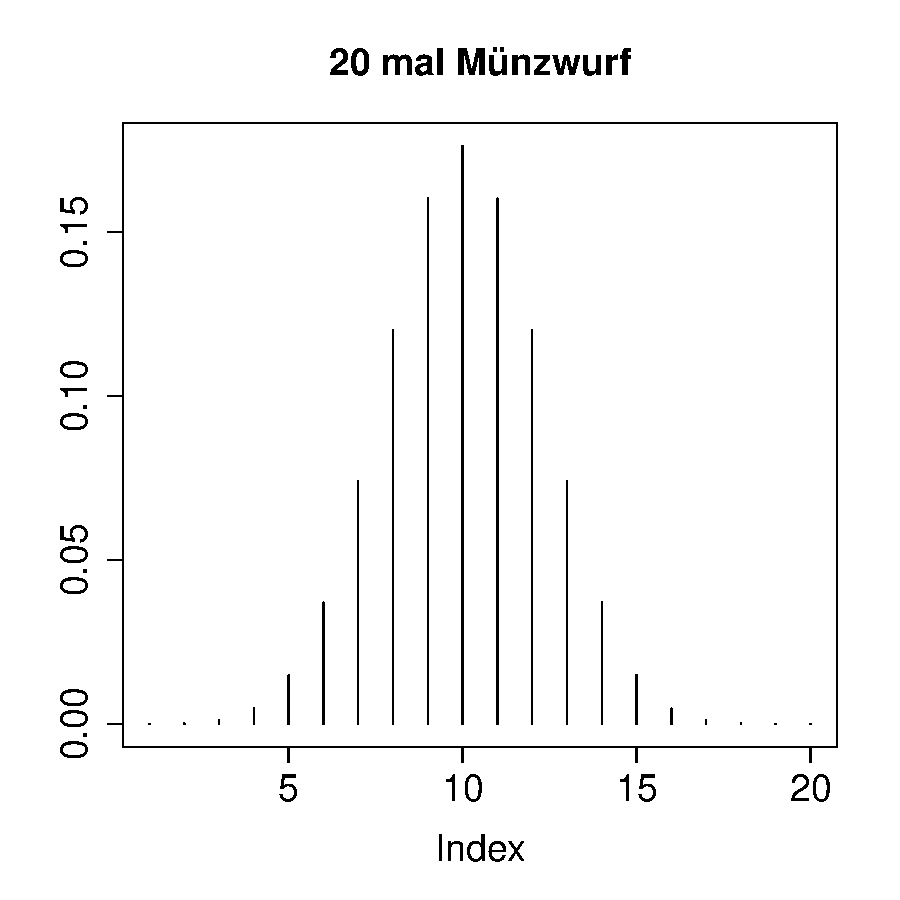
\includegraphics{verteilungen-026}
\caption{Verteilung für 20 Versuche}
\end{subfigure}
\caption{Wahrscheinlichkeitsverteilung beim Münzwurf}
\end{figure}

\clearpage
\newpage
\section{Poissonverteilung}

\subsection{Verwendung in R}
\lstinline{R} stellt grundsätzlich vier Funktionen für die 
Poissonverteilung zur Verfügung. 
\begin{itemize}
	\item \lstinline{dpois()} \hfill{} 
		(\emph{Wahrscheinlichkeitsverteilung})
	\item \lstinline{pois()} \hfill{}
		(\emph{kumulative Wahrscheinlichkeit})
	\item \lstinline{qpois()} \hfill{}
		(\emph{Verteilung der Quantile})
	\item \lstinline{rpois()} \hfill{}
		(\emph{Zufallszahlen})
\end{itemize}





\begin{figure}[h!]
\centering
\begin{subfigure}[b]{0.48\textwidth}
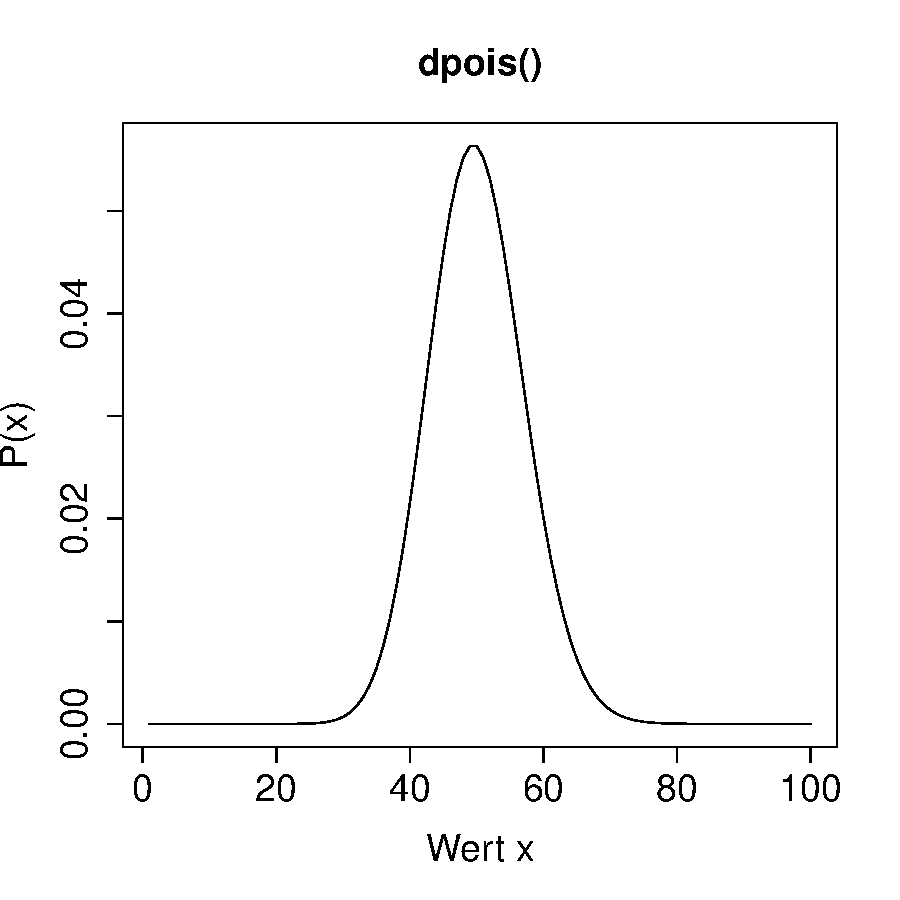
\includegraphics{verteilungen-031}
\caption{Wahrscheinlichkeitsverteilung}
\end{subfigure}
\begin{subfigure}[b]{0.48\textwidth}
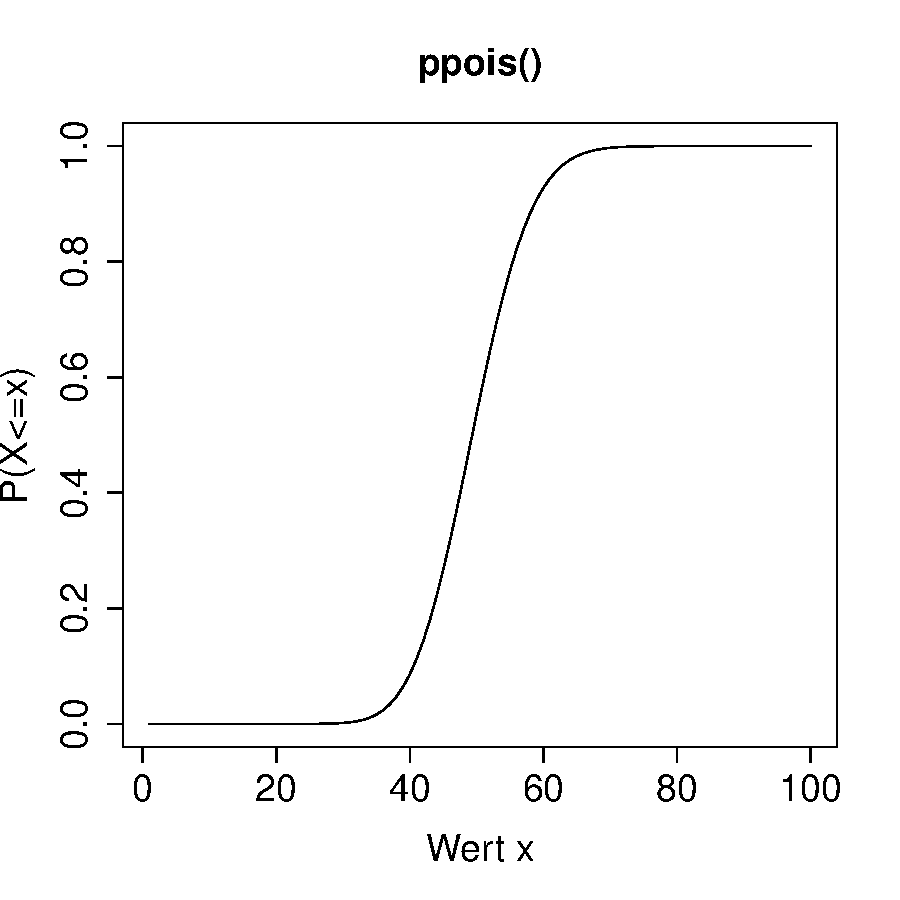
\includegraphics{verteilungen-032}
\caption{kumulative Wahrscheinlichkeit}
\end{subfigure}

\begin{subfigure}[b]{0.48\textwidth}
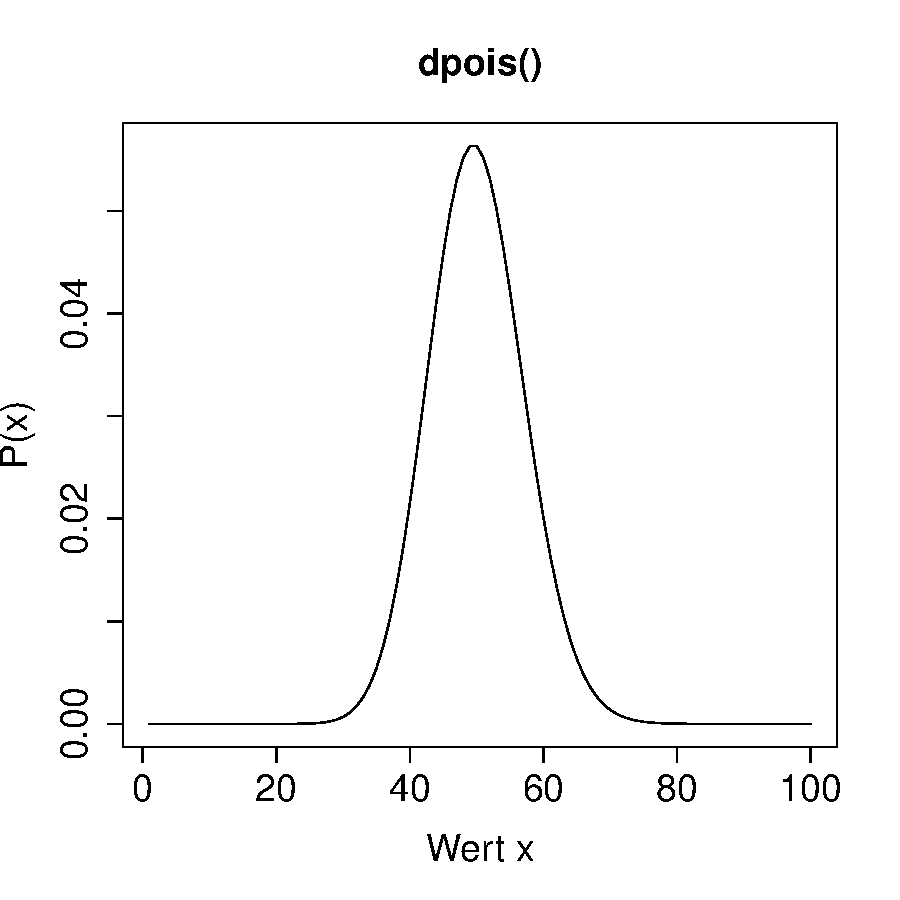
\includegraphics{verteilungen-033}
\caption{Quantile}
\end{subfigure}
\begin{subfigure}[b]{0.48\textwidth}
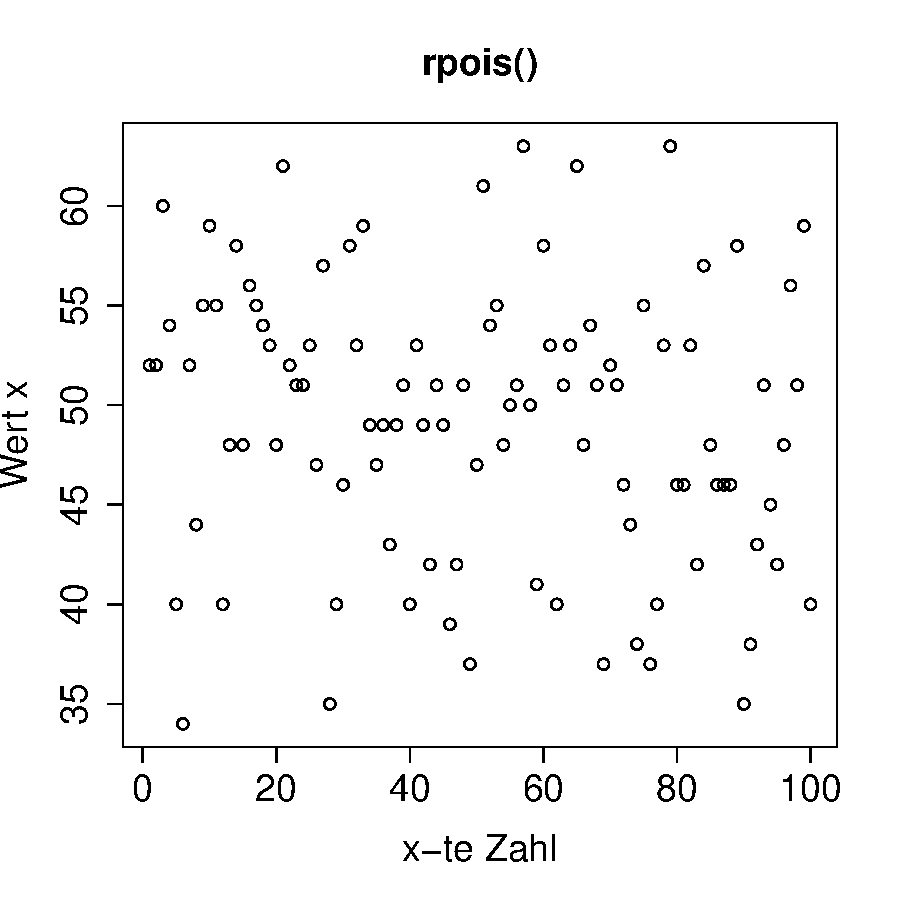
\includegraphics{verteilungen-034}
\caption{Zufallszahlen}
\end{subfigure}
\caption{Poissonverteilung ($\lambda=50$)}
\end{figure}

\clearpage

\section{Erwartungswert}
Der Erwartungswert einer diskreten Verteilung gibt jene Zahl an,
welche die Zufallsvariable im \emph{Mittel} annimmt. Sie beschreibt
quasi den mittleren Wert der Verteilung.

Für diskrete Wahrscheinlichkeitsverteilungen gilt, dass der 
Erwartungswert der Summe von Produkten aus Wahrscheinlichkeit und
Wert der Zufallsvariable entspricht. 
\[ \mu = E(X) = \sum x \cdot P(X=x) \]
$P(X=x)$ bedeutet \emph{Wahrscheinlichkeit, dass die Zufallsvariable $X$ 
genau $x$ ist}.


\section{Varianz}
Die Varianz einer Wahrscheinlichkeitsverteilung gibt ein Mass an für 
die Streuung der Warscheinlichkeiten um den Erwartungswert.

Die Varianz wird analog zum Erwartungswert ermittelt, wobei der Wert
der Zufallsvariable $x$ ersetzt wird durch das Quadrat der Abweichung
von Zufallsvariable und Erwartungswert $(x-\mu)^2$
\[ \begin{array}{l c l}
	Var(X) 
		& = 
		& E(X-\mu)^2 \\
	& &  \\
	Var(X)
		& = 
		& \sum \left( (x-\mu)^2 \cdot P(X=x) \right)
\end{array} \]

\section{Standardabweichung}
Die Standardabweichung einer Wahrscheinlichkeitsverteilung 
ist wie die Varianz ein Mass für die Streuung. Sie 
wird anhand der Varianz ermittelt mit dem Zusammenhang, dass die 
Standardabweichung der Quadratwurzel der Varianz entspricht.
\[ \begin{array}{l c l} 
	\sigma 
		& = 
		& \sqrt{Var(X)} \\
	& & \\
	\sigma
		& =
		& \sqrt{E(X-\mu)^2} \\
	& & \\
	\sigma
		& =
		& \sqrt{\sum \left( (x-\mu)^2 \cdot P(X=x) \right)}
\end{array} \]

\section{Zusammenfassung}

\subsection{Erwartungswert und Varianz}

\begin{table}[h!]
	\centering
	\begin{tabular}{l c c}
		Verteilung
			& $E(X)$
			& $Var(X)$ \\
		\hline
		& & \\
		$X \sim Hyp(n,r,s)$
			& $n \cdot \left(\frac{r}{N}\right)$
			& $n \cdot \left( 
				\frac{r}{N}
				\right) 
			\left( 
				1 - \frac{r}{N}
			\right)
			\left(
				\frac{(N)-n}{(N)-1}
			\right)$ \\
		& & \\
		$X \sim Bin(n,p)$
			& $n \cdot p$
			& $n \cdot p \cdot (1-p)$ \\
		& & \\
		$X \sim Pois(\lambda)$
			& $\lambda$
			& $\lambda$
	\end{tabular}
\end{table}

\subsection{Berechnungen in R}

\begin{table}[h!]
	\begin{tabular}{l l l}
	Hypergeometrisch & & \\ \hline
		& genau 	& \verb!dhyper(x=A,...)! \\
		& höchstens 	& \verb!phyper(q=A,...)! \\
		& mindestens 	& \verb!1-phyper(q=A-1,...)! \\
		& zufällig 	& \verb!rhyper(n=...)! \\
	& & \\
	Binomial & & \\ \hline
		& genau 	& \verb!dbinom(x=A,...)! \\
		& höchstens 	& \verb!pbinom(q=A,...)! \\
		& mindestens 	& \verb!1-pbinom(q=A-1,...)! \\
		& zufällig 	& \verb!rbinom(n=...)! \\
	& & \\
	Poisson & & \\ \hline
		& genau 	& \verb!dpois(x=A,...)! \\
		& höchstens 	& \verb!phyper(q=A,...)! \\
		& mindestens 	& \verb!1-ppois(q=A-1,...)! \\
		& zufällig 	& \verb!rpois(n=...)! \\
	\end{tabular}
\end{table}

\chapter{Stetige Verteilungen}
Stetige und absolut stetige Verteilungen beschreibebn Probleme, 
welche Ergebnisse aus $\mathbb{R}$ liefern.

\paragraph{Stetig} Die Eigenschaft der Stetigkeit ist so definiert,
dass die Punktwahrscheinlichkeit einer Zufallsvariable 
$X$ Null ergibt und $x$ auch wirklich jeden Wert aus
$\mathbb{R}$ annehmen kann.
\[ 
	P(X=x) = 0, \qquad x\in\mathbb{R}
\]
\paragraph{Absolute Stetigkeit}
Als absolut stetig werden Funktionen beschrieben die integrierbar 
sind. 

\newpage

\section{Dichtefunktion}
Die Dichtefunktion $f(x)$ ist definiert als die Ableitung der kummulativen
Verteilungsfunktion $F(x)$.
\[  
	\int f(x) := F(x) 
		\qquad 
		\Leftrightarrow 
		\qquad 
		f(x) = \frac{d}{dx} F(x)
		= F'(x)
\]
Mit der Dichte lässt sich eine Aussage darüber treffen, wie die 
Wahrscheinlichkeit ist, dass eine Zufallsvariable $X$ einen Wert
in einem bestimmten Intervall $[a,b]$ annimmt (siehe Grafik 
\ref{fig:dichte}).

\begin{figure}[h!]
	\centering
	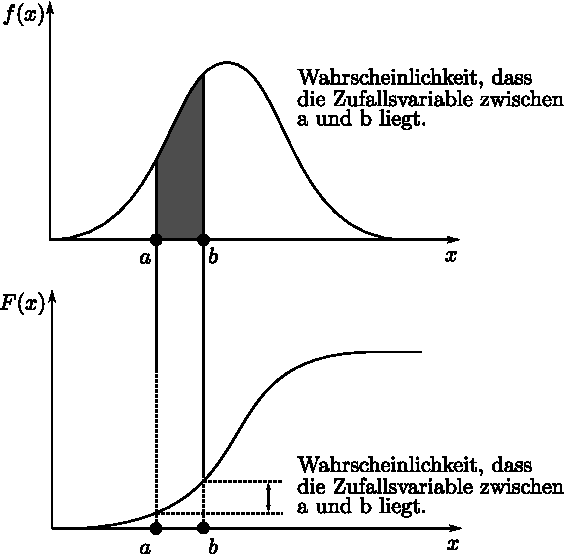
\includegraphics[width=0.7\textwidth]{dichtefunktion.pdf}
	\caption{Dichtefunktion $f(x)$ und kummulative Verteilungsfunktion 
		$F(x)$ in der Gegenüberstellung.}
	\label{fig:dichte}
\end{figure}

Mit der Definition der Dichtefunktion $f(x)$ lassen sich mehrere 
Gesetzmässigkeiten herleiten:
\begin{itemize}
	\item Die Dichte in einem Punkt $a$ ist Null.
		\[ f(x) = 0 
			\qquad \lim_{a_1 \rightarrow a_0} \left(
				\int_{a_0}^{a_1} f(x)\,dx \right) = 0   \]
	\item Das Integral einer Dichtefunktion über einem Intervall
		$[a,b]$ ist gleich der Differenz der kummulativen
		Wahrscheinlichkeiten von $a$ und $b$ (siehe Grafik 
		\ref{fig:dichte}).
		\[ \int_a^b f(X)\, dx = F(b) - F(a) \]
	\item Das Integral der Dichtefunktion über dem Intervall 
		$[-\infty, +\infty]$ ist genau 1 
		(siehe \gls{Axiome von Kolmogorov}, \gls{Normiertheit}).
		Dies bedeutet, dass die kummulative Verteilungsfunktion
		für grosse $x$ gegen $1$ strebt und für kleine gegen $0$.
		\[ \int_{-\infty}^{+\infty} f(x)\, dx = 1 \]
		\[ F(x) \xrightarrow{x \rightarrow +\infty} 1
			\qquad \Leftrightarrow \qquad 
			\lim_{x \rightarrow + \infty} 
				F(x) = 1 \]
		\[ F(x) \xrightarrow{x \rightarrow -\infty} 0 
			\qquad \Leftrightarrow \qquad
			\lim_{x \rightarrow - \infty} 
				F(x) = 0 \]
\end{itemize}

\subsection{Erwartungswert}
Der Erwartungswert einer stetigen Verteilung mit der Dichte $f(x)$ und 
der Funktion g(x) ist allgemein definiert als
\[ 
	E(g(X)) = \int_{-\infty}^{+\infty} g(x) \cdot f(x)\, dx
\]
Falls die Funktion $g(x)$ mit einer Variable gleichgesetzt werden
kann, also $g(x)=x$ gilt, dann kann der Erwartungswert auch berechnet
werden als
\[  
	E(X) = \int_{-\infty}^{+\infty} x \cdot f(x)\, dx,
		\qquad x = g(x)
\]

\subsection{Varianz}
\[ \begin{array}{l c l} 
	Var(X) 
		& = 
		& \displaystyle 
			\int_{-\infty}^{+\infty} 
			(x-E(X))^2 \cdot f(x)\, dx \\
		& & \\
		& = 
		& E(X-E(X))^2 \\
		& & \\
		& = 
		& E(X^2) - E(X)^2
\end{array} \]

\subsection{Standardabweichung}
Die Standardabweichung wird wie bei den diskreten Verteilungen 
duch die Wurzel aus der Varianz ermittelt.
\[  
	\sigma_x = \sqrt{Var(X)}
\]

\subsection{Quantile}
Ein Quantil $q(\alpha)$ markiert (in \%) die $x$-Stelle einer 
Dichtefunktion $f(x)$, bei welcher der angegebene Anteil $\alpha$
darunter liegt.
\[ 
	q(\alpha), 
		\qquad \alpha = 
		\{x \mid 0 < x < 1 \land x \in \mathbb{R}\}
\]
\[
	P(X \leq q(\alpha)) = \alpha
\]
\[ 
	F(q(\alpha)) = \alpha  
		\qquad \Leftrightarrow \qquad
		F^{-1}(\alpha) = q(\alpha)
\]

\begin{figure}[h!]
	\centering
	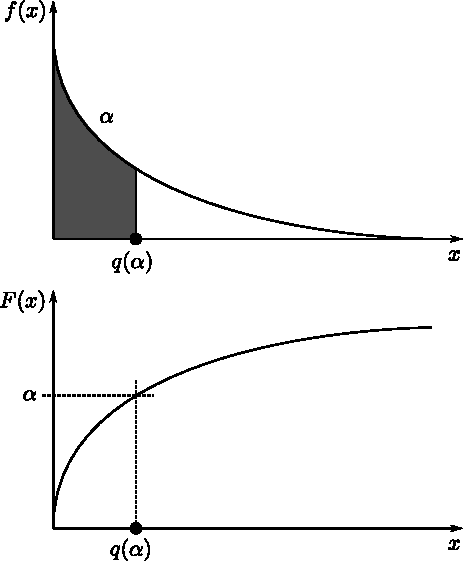
\includegraphics[width=0.7\textwidth]{dichtefunktion-quantile.pdf}
	\caption{Quantil einer Dichtefunktion.}
	\label{fig:dichte-quantil}
\end{figure}

\clearpage
\newpage
\section{Uniforme Verteilung}

Die uniforme Verteilung (auch \emph{Gleichverteilung}) ist eine
Verteilung, deren Wahrscheinlichkeit nur in einem bestimmten 
Intervall $[a,b]$ ungleich Null ist. Die Dichte $f(x)$ innerhalb 
des Intervalls $[a,b]$ ist konstant und ausserhalb davon gleich Null.
Zusammenfassend kann man sagen, dass die uniforme Verteilung eine
konstante Dichte hat.

\[  
	f(x) = \mathrm{konstant} = \left\{\begin{array}{c c l}
		\displaystyle \frac{1}{b-a}
			& \text{falls}
			& a < x < b \\
		& & \\
		0
			& \text{falls}
			& (x < a) \lor (x > b)
		\end{array} \right.
\]

\begin{figure}[h!]
	\centering
	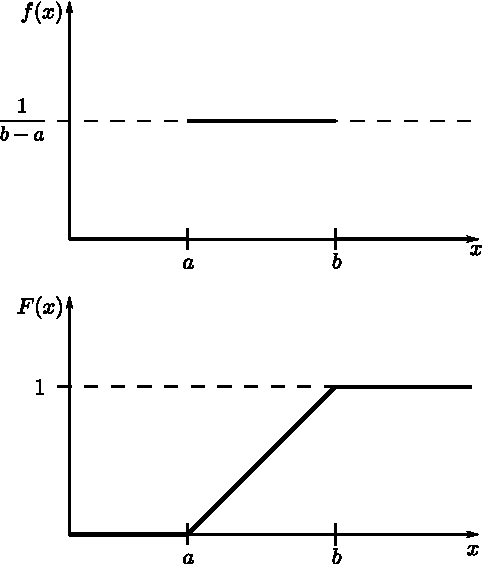
\includegraphics[width=0.7\textwidth]{uniform.pdf}
	\caption{Uniforme Dichte $f(x)$ und Verteilung $F(x)$.}
	\label{fig:uniform}
\end{figure}

\subsection{Verteilungsfunktion}
Die Verteilungsfunktion der uniformen Verteilung beschreibt
grundsätlich eine Gerade und wenn das Intervall 
$[a,b]\neq[-\infty, +\infty]$ ist, so ist diese Bereichsweise
definiert.

\[  
	F(x) = \left\{
		\begin{array}{c c l}
			0 
				& \text{falls } 
				& x < a \\
			& \\
			\displaystyle
			\frac{x-a}{b-a} 
				& \text{falls } 
				& a < x < b \\
			& \\
			1
				& \text{falls } 
				& b < x
		\end{array} \right.
\]

\subsection{Erwartungswert}
Da die Dichtefunktion der uniformen Verteilung konstant ist,
kann der Erwartungswert sehr einfach berechnet werden.
\[  
	E(X) = \frac{a+b}{2}
\]
Die Werte $a,b$ können auch als Minimal- bzw. Maximalwerte
betrachtet werden.
\[  
E(X) = \frac{\text{min} + \text{max}}{2}
\]

\subsection{Varianz}
Analog zum Erwartungswert ist auch die Berechnung der Varianz
einer uniformen Verteilung relativ einfach.
\[ 
	Var(X) = \frac{(b - a)^2}{12}
\]
Wie auch beim Erwartungswert, können die Intervallgrenzen
$[a,b]$ als Mininal- und Maximalwerte betrachtet werden.
\[  
	Var(X) = \frac{(\text{max} - \text{min})^2}{12}
\]

\subsection{Verwendung in R}
\lstinline{R} stellt grundsätzlich vier Funktionen für die 
uniforme Verteilung zur Verfügung. 
\begin{itemize}
	\item \lstinline{dunif()} \hfill{} 
		(\emph{Wahrscheinlichkeitsverteilung})
	\item \lstinline{punif()} \hfill{}
		(\emph{kumulative Wahrscheinlichkeit})
	\item \lstinline{qunif()} \hfill{}
		(\emph{Verteilung der Quantile})
	\item \lstinline{runif()} \hfill{}
		(\emph{Zufallszahlen})
\end{itemize}
Die Abbildung \ref{fig:unif} zeigt jeweils einen Plot zu den gegebenen
Funktionen aus \lstinline{R}. Für weitere Informationen zu Plots siehe
Kapitel \ref{sec:plots}.





\begin{figure}[h!]
\centering
\begin{subfigure}[b]{0.48\textwidth}
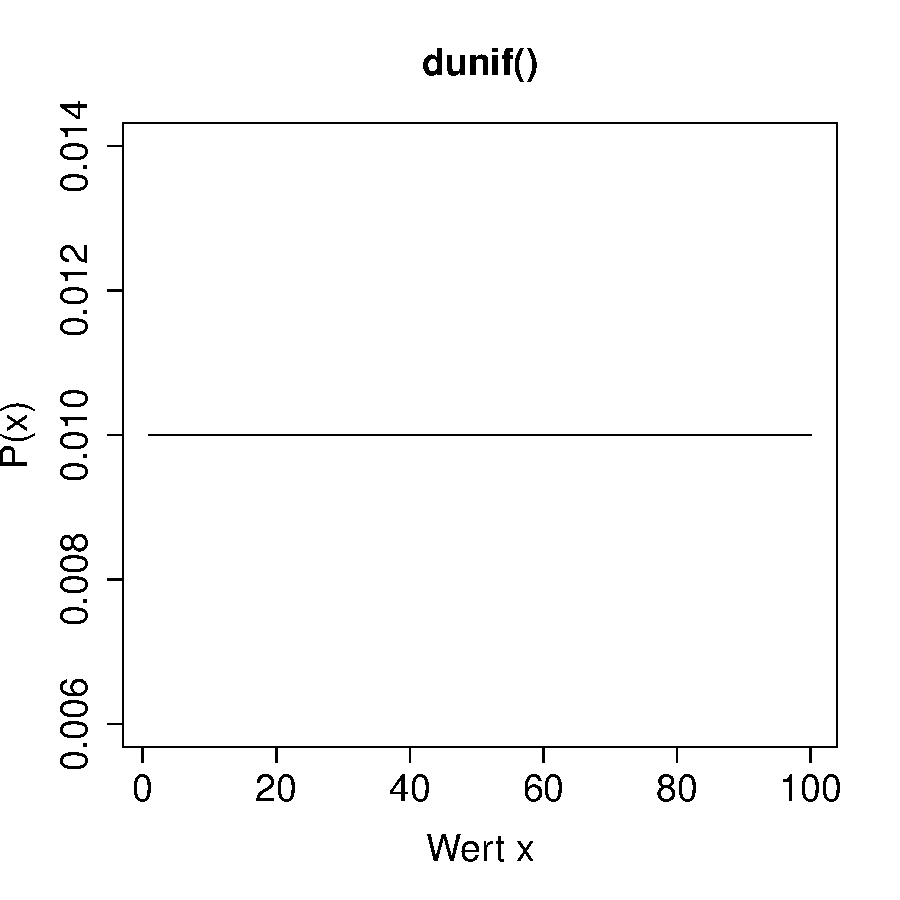
\includegraphics{verteilungen-039}
\caption{Wahrscheinlichkeitsverteilung}
\end{subfigure}
\begin{subfigure}[b]{0.48\textwidth}
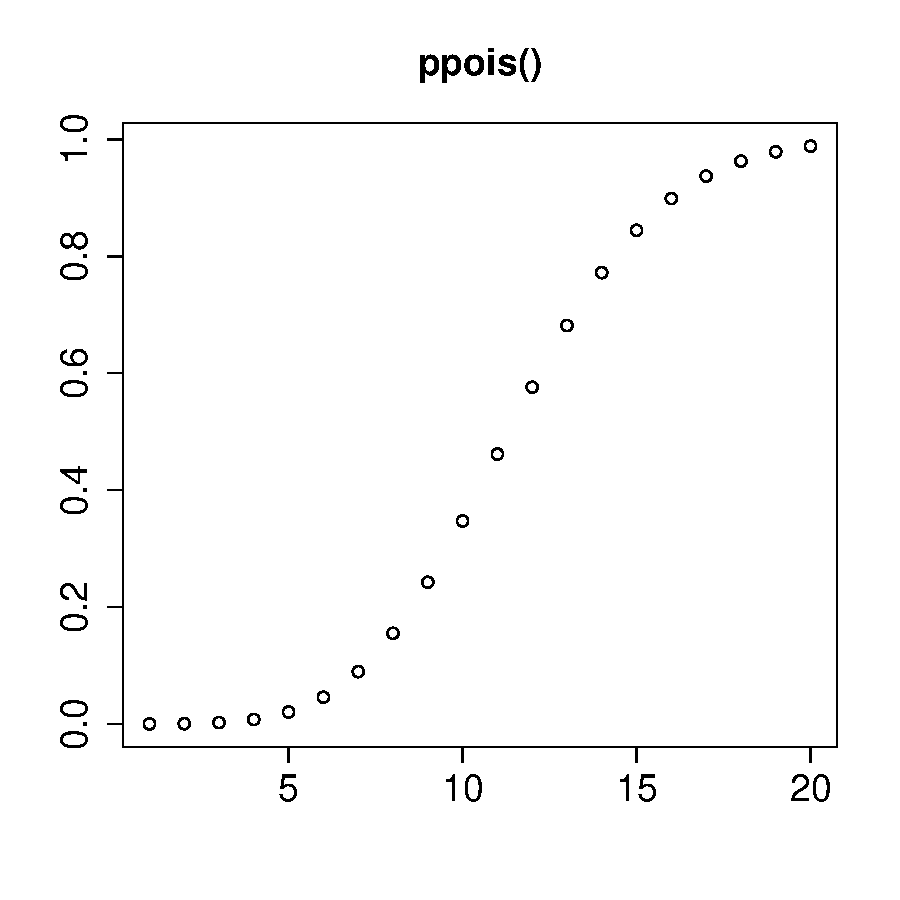
\includegraphics{verteilungen-040}
\caption{kumulative Wahrscheinlichkeit}
\end{subfigure}

\begin{subfigure}[b]{0.48\textwidth}
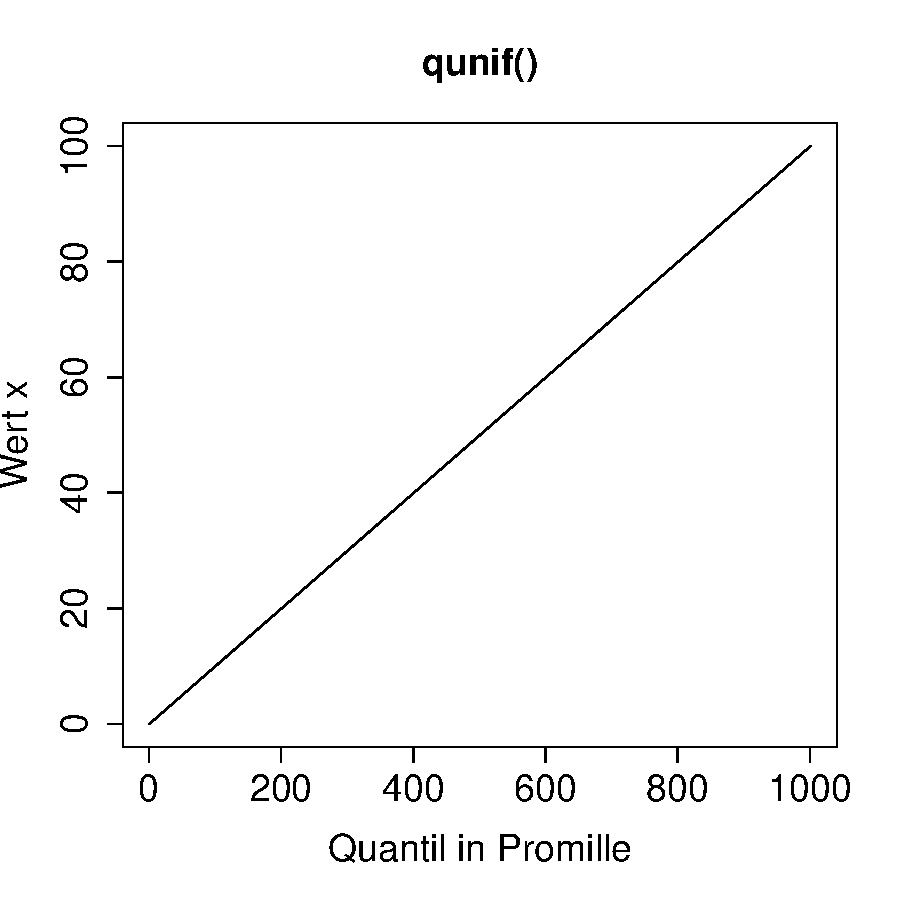
\includegraphics{verteilungen-041}
\caption{Quantile}
\end{subfigure}
\begin{subfigure}[b]{0.48\textwidth}
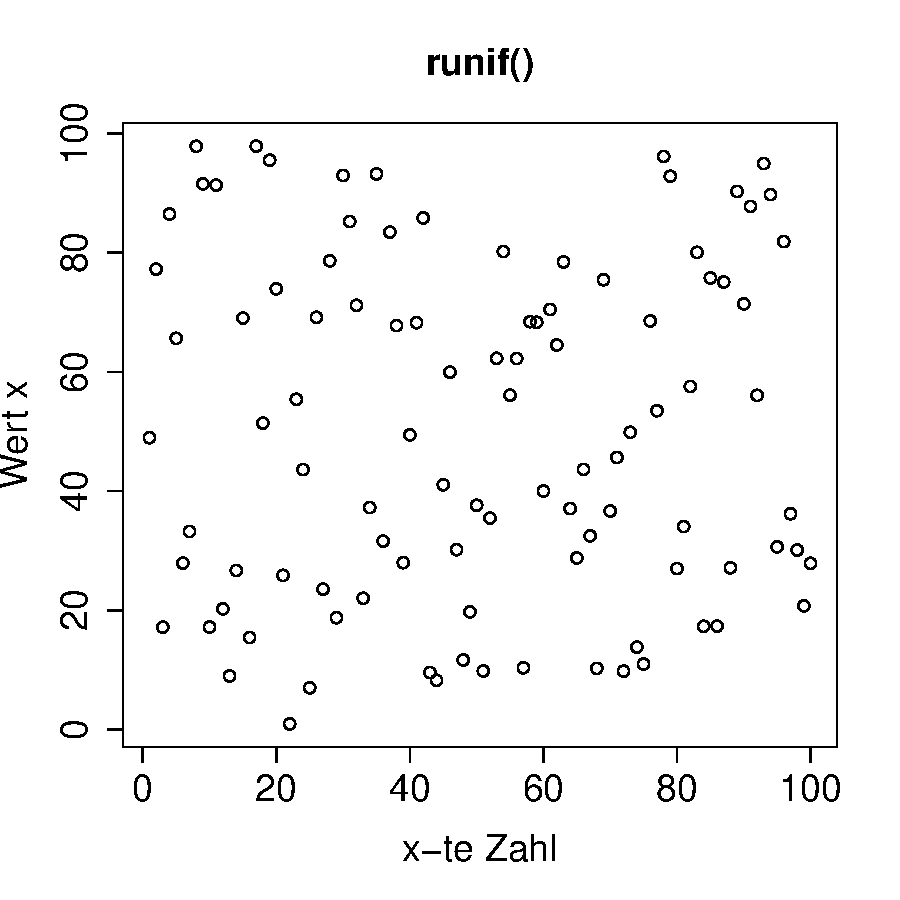
\includegraphics{verteilungen-042}
\caption{Zufallszahlen}
\end{subfigure}
\caption{Uniforme Verteilung ($n=100, min=0, max=100$)}
\label{fig:unif}
\end{figure}

\clearpage
\subsection{Beispiel einer uniformen Verteilung}
Benutzt man einen ADC (engl. \emph{Analog to Digital Converter}) zur 
Erfassung elektronischer Messgrössen als digitale Werte, so 
\emph{quantifziert} dieser die Messung und es entsteht ein Messfehler. 
Ist die zu erfassende Grösse viel grösser als die kleinstmögliche 
Auflösung des ADC, so ist dieser Fehler uniform verteilt.

\begin{Schunk}
\begin{Sinput}
> f1 <- 10*sin(x=seq(0, 2*pi, 0.001))
> adc.in  <- (f1)
> adc.out <- round(x=adc.in, digits=0)
> error   <- (adc.in - adc.out)
> m <-mean(error)
> s <-sd(error)
> m
\end{Sinput}
\begin{Soutput}
[1] -0.0001592544
\end{Soutput}
\begin{Sinput}
> s
\end{Sinput}
\begin{Soutput}
[1] 0.27766
\end{Soutput}
\end{Schunk}

Mit Hilfe von R lässt sich dieses Beispiel relativ leicht rechnen und
plotten (siehe \ref{fig:adc}). Die Plots zeigen, dass die Quantifizireung
des Eingangsignal einen uniformen Fehler verusrsacht. Dies ist durch
den QQ-Plots explizit dargestellt, welcher die Quantile einer Datenreihe
mit uniformer Verteilung vergleicht mit den Quantilen der Messfehler.





\begin{figure}[h!]
\centering
\begin{subfigure}[b]{0.48\textwidth}
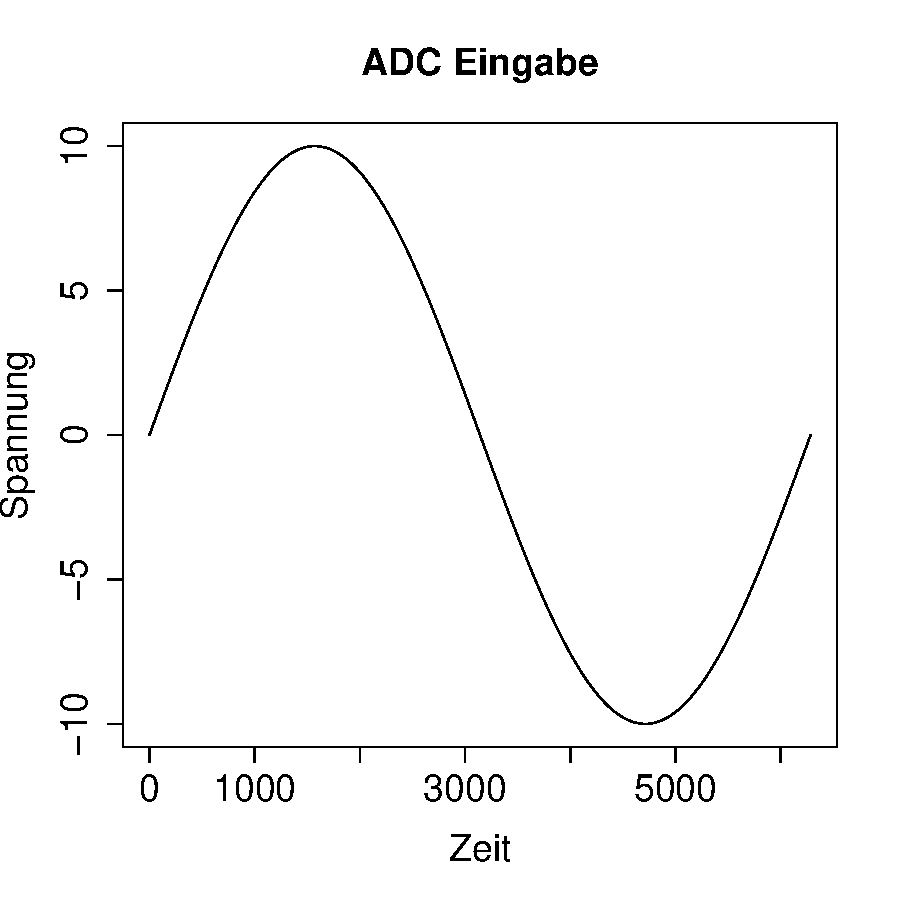
\includegraphics{verteilungen-048}
\caption{Eingangssignal $u_e(t)\in\mathbb{R}$}
\end{subfigure}
\begin{subfigure}[b]{0.48\textwidth}
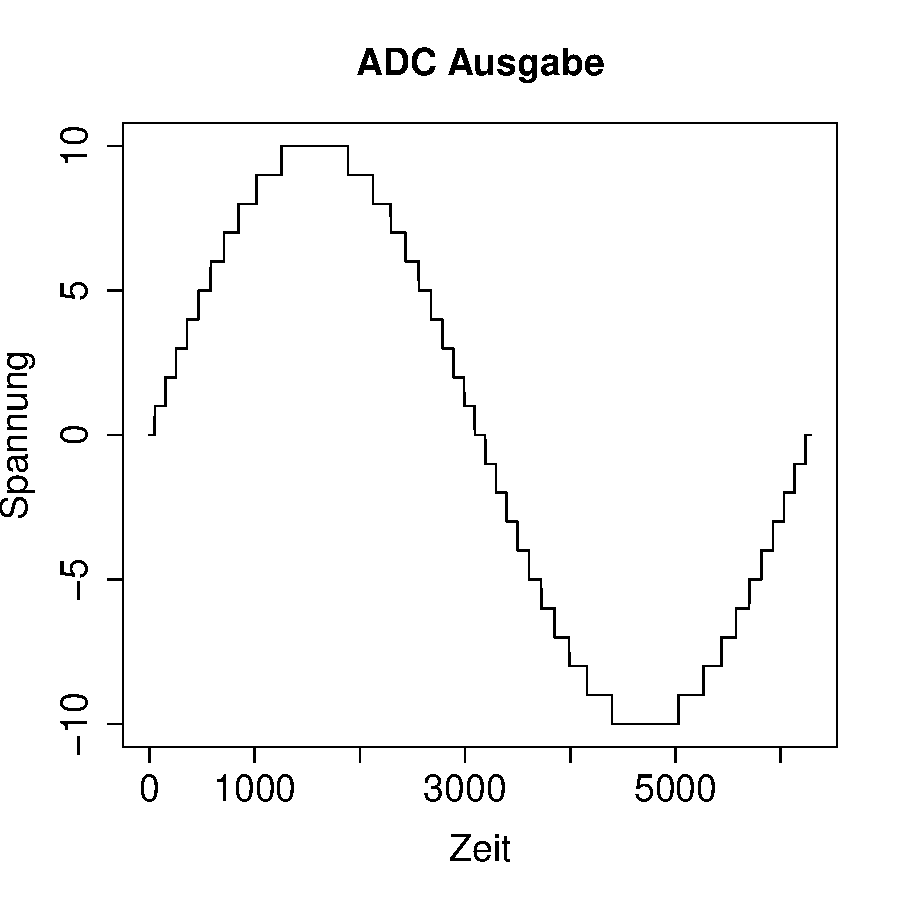
\includegraphics{verteilungen-049}
\caption{Digitalisierung $(\mathbb{R} \rightarrow 2^n, n\in \mathbb{N})$}
\end{subfigure}

\begin{subfigure}[b]{0.48\textwidth}
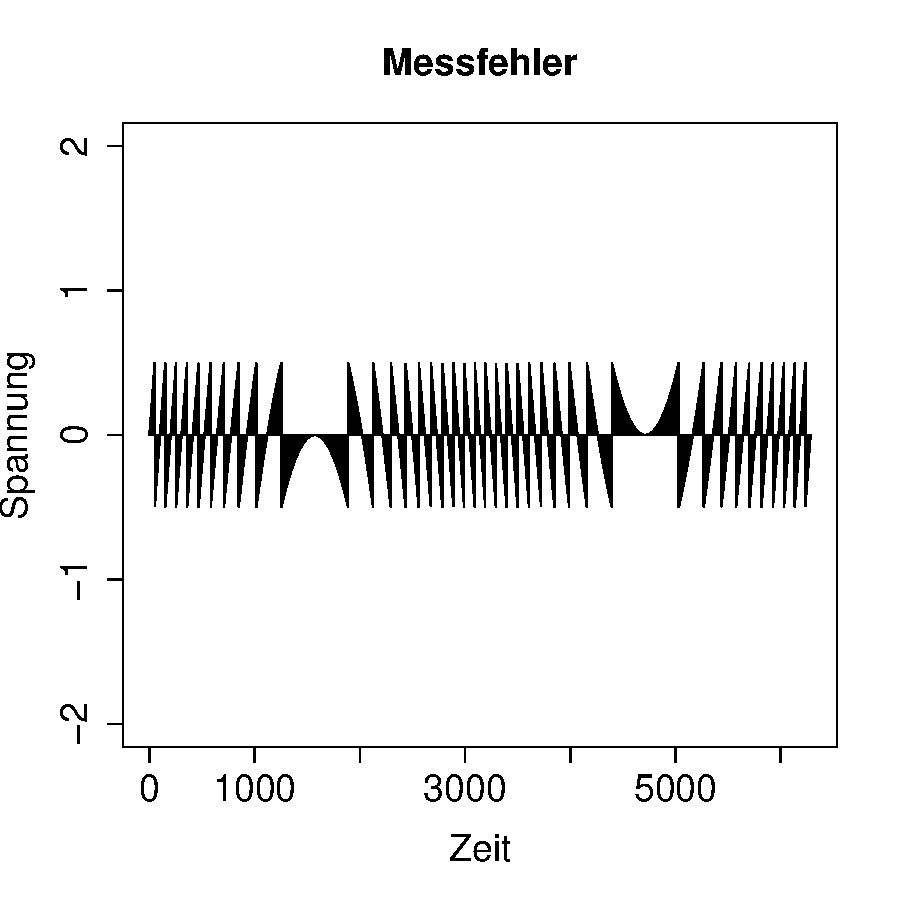
\includegraphics{verteilungen-050}
\caption{Fehler $u_a(t)$}
\end{subfigure}
\begin{subfigure}[b]{0.48\textwidth}
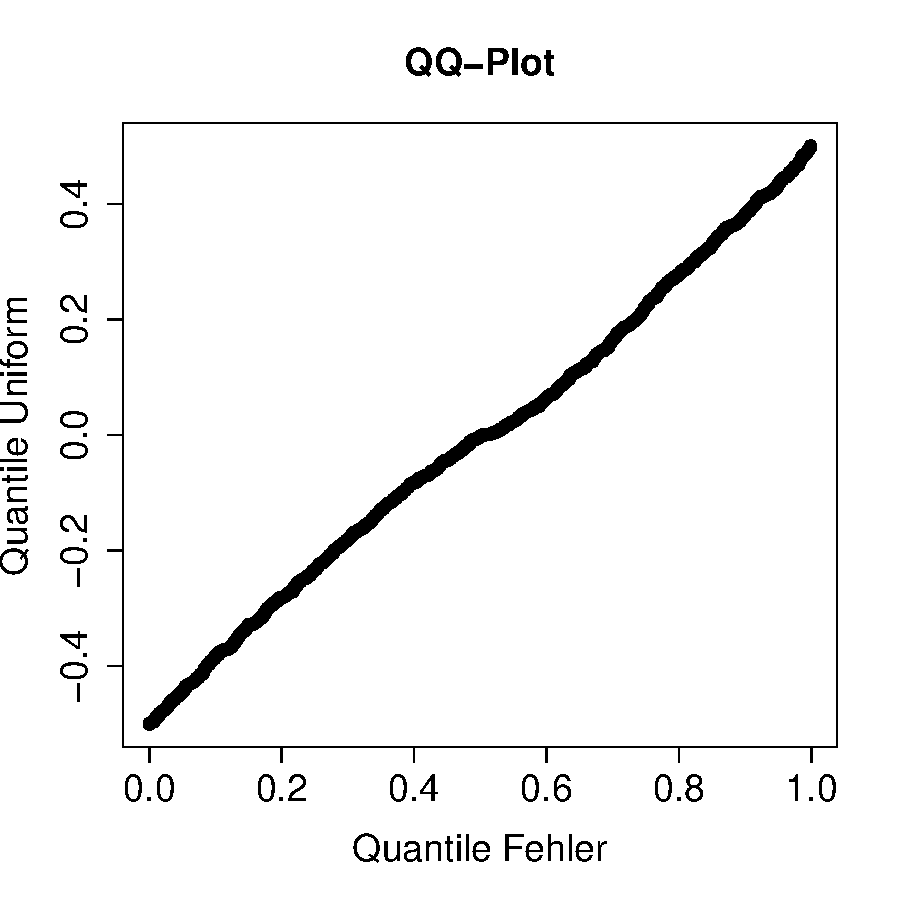
\includegraphics{verteilungen-051}
\caption{Quantilenvergleich mit $\mathcal{U}(a,b)$}
\end{subfigure}
\caption{Quantifizierungfehler eines ADC.}
\label{fig:adc}
\end{figure}

\newpage
\section{Normalverteilung}
\subsection{Verteilungsfunktion}
\subsection{Erwartungswert}
\subsection{Varianz}
\subsection{Verwendung in R}
\subsection{Beispiel einer Normalverteilung}

\newpage
\section{Exponentialverteilung}
\subsection{Verteilungsfunktion}
\subsection{Erwartungswert}
\subsection{Varianz}
\subsection{Verwendung in R}
\subsection{Beispiel einer Exponentialverteilung}

\newpage
\section{Zusammenfassung}
\paragraph{Uniforme Verteilung}
\[ X \sim \mathcal{U}(a,b) \]
\[ \begin{array}{l c l}
	F(X) 
		& =
		& \displaystyle \frac{x-a}{b-a} \\
	f(x)	
		& =
		& \displaystyle \frac{1}{b-a}  \\
	D_f	
		& = 
		& a < x < b \\
	E(X)
		& = 
		& \displaystyle \frac{a+b}{2}\\
	Var(X)	
		& =
		& \displaystyle \frac{(b-a)^2}{12}\\
\end{array} \]

\paragraph{Normalverteilung}
\[ X \sim \mathcal{N}(\mu, \sigma^2) \]
\[ \begin{array}{l c l}
	F(X) 
		& =
		& \displaystyle \frac{x-a}{b-a} \\
	f(x)	
		& =
		& \displaystyle \frac{1}{\sigma\sqrt{2\pi}} \cdot
				e^{\left(
					-\frac{(x-\mu)^2}{2\sigma^2}
				\right)} \\
	D_f	
		& = 
		& x \in \mathbb{R} \\
	E(X)
		& = 
		& \mu\\
	Var(X)	
		& =
		& \sigma^2 \\
\end{array} \]

\paragraph{Exponentialverteilung}
\[ X \sim Exp(\lambda) \]
\[ \begin{array}{l c l}
	F(X) 
		& =
		& F(X) = \displaystyle \frac{x-a}{b-a} \\
	f(x)	
		& =
		& \displaystyle \lambda \cdot 
				e^{\left(
					-\lambda x
				\right)} \\
	D_f	
		& = 
		& x > 0 \\
	E(X)
		& = 
		& \displaystyle \frac{a+b}{2}\\
	Var(X)	
		& =
		& \displaystyle \frac{(b-a)^2}{12}\\
\end{array} \]


\subsection{Berechnungen in R}
